\documentclass[a4paper,twocolumn]{article}


\usepackage[sc]{mathpazo} % Use the Palatino font
\usepackage[T1]{fontenc} % Use 8-bit encoding that has 256 glyphs
\usepackage[utf8]{inputenc} % Use utf-8 as encoding
\linespread{1.05} % Line spacing - Palatino needs more space between lines
\usepackage{microtype} % Slightly tweak font spacing for aesthetics

\usepackage[spanish]{babel} % Language hyphenation and typographical rules
%\usepackage[galician]{babel} % Change to this if using galician

\usepackage[hmarginratio=1:1,top=32mm,columnsep=20pt]{geometry} % Document margins
\usepackage[hang, small,labelfont=bf,up,textfont=it,up]{caption} % Custom captions under/above floats in tables or figures
\usepackage{booktabs} % Horizontal rules in tables
\usepackage{float} % For [H] float option
\usepackage{abstract} % Allows abstract customization
\renewcommand{\abstractnamefont}{\normalfont\bfseries} % Set the "Abstract" text to bold
\renewcommand{\abstracttextfont}{\normalfont\small\itshape} % Set the abstract itself to small italic text

\usepackage{titlesec} % Allows customization of titles
\renewcommand\thesection{\Roman{section}} % Roman numerals for the sections
\renewcommand\thesubsection{\Alph{subsection}} % roman numerals for subsections
\titleformat{\section}[block]{\large\scshape\centering}{\thesection.}{1em}{} % Change the look of the section titles
\titleformat{\subsection}[block]{\large}{\thesubsection.}{1em}{} % Change the look of the section titles

\usepackage{fancyhdr} % Headers and footers
\pagestyle{fancy} % All pages have headers and footers
\fancyhead{} % Blank out the default header
\fancyfoot{} % Blank out the default footer
%\fancyhead[C]{Running title $\bullet$ May 2016 $\bullet$ Vol. XXI, No. 1} % Custom header text
\fancyfoot[C]{\thepage} % Custom footer text

\usepackage{titling} % Customizing the title section

\usepackage{hyperref} % For hyperlinks in the PDF

\usepackage{graphicx}

\usepackage{amsmath}
 
%----------------------------------------------------------------------------------------
%	TITLE SECTION
%----------------------------------------------------------------------------------------
 
\setlength{\droptitle}{-4\baselineskip} % Move the title up

\pretitle{\begin{center}\huge\bfseries} % Article title formatting
	\posttitle{\end{center}} % Article title closing formatting

\title{Clasificación de Arritmias Cardíacas mediante Aprendizaje Automático: Análisis de Señales ECG} % Article title

\author{%
	\textsc{Juan Manuel} \\[1ex] % Your name
	\normalsize Matemáticas y Estadística para la IA\\
	\normalsize Grupo 1 \\ % Your institution
	\normalsize jantofer@myuax.com % Your email address
	%\and % Uncomment if 2 authors are required, duplicate these 4 lines if more
	%\textsc{Jane Smith}\thanks{Corresponding author} \\[1ex] % Second author's name
	%\normalsize University of Utah \\ % Second author's institution
	%\normalsize \href{mailto:jane@smith.com}{jane@smith.com} % Second author's email address
}
\date{\today} % Leave empty to omit a date
\renewcommand{\maketitlehookd}{%
	\begin{abstract}
		\noindent En este trabajo se desarrolla un sistema de detección de arritmias cardíacas basado en el análisis de señales electrocardiográficas (ECG), con el objetivo de construir un wearable de monitorización para mayores de 60 años. 
		Con este fin, se partió de la base de datos MIT-BIH, compuesta por 87,554 registros de entrenamiento y 21892 de validación, a partir de los cuales se implementó un pipeline que comenzó con una caracterización de patrones ECG mediante
		 estadísticas descriptivas y visualización de señales, reducción dimensional mediante Análisis de Componentes Principales (PCA), y construcción de dos modelos de clasificación supervisada. Se implementaron dos enfoques a través de clasificación binaria: un árbol de 
		 decisión, y clasificador Naive-Bayes gaussiano, cuyos resultados, a pesar de que han mostrado los conflictos propios del solapamiento de clases, han podido demostrar la viabilidad de este tipo de sistemas de apoyo al diagnóstico 
		 con una fiabilidad aceptable. 
		\\\mbox{}\\
		 \textbf{\textit{Palabras clave}: Arritmias cardíacas, Clasificación de latidos, señales ECG, Aprendizaje automático, Análisis de Componentes Principales (PCA), Naive-Bayes, Árbol de decisión.}
	\end{abstract}
}

%----------------------------------------------------------------------------------------

% \begin{document}
	
% 	% Print the title
% 	\maketitle
	
% 	%----------------------------------------------------------------------------------------
% 	%	ARTICLE CONTENTS
% 	%----------------------------------------------------------------------------------------
	
% 	\section{Introducción}
	
% 	Introducción al problema tratado, incluyendo las referencias  necesarias. Por ejemplo: ``Este trabajo se basa en los estudios teóricos realizados en~\cite{Intel:2005} y \cite{spec}". En este apartado se plantean el problema a resolver, objetivos a alcanzar y metodología seguida para alcanzarlos.
	
% 	Es una introducción al problema, no se desarrollarán los contenidos aquí. 
	
% 	La introducción termina indicando en pocas palabras de qué secciones consta el resto del documento y de qué trata cada una. Se mencionan todas las secciones salvo la de referencias (bibliografía). 

% 	%------------------------------------------------
	
% 	\section{Nombre del apartado}
% 	Puede haber tantas secciones como sea necesario para presentar el trabajo pero no más de 4 o 5. Siempre se les pone un nombre que haga referencia al contenido. 
	
% 	Se entra en materia indicando en nuestro caso qué tipo de información vamos a analizar y porqué, así como de donde la hemos obtenido. 
	
% 	Esta sección explica la metodología que hemos usado, por ejemplo el uso de benckmarks, de que tipo son y para que se usan
	
% 	Esta sección puede estar dividida en varias subsecciones. 
	
% 	El cuadro~\ref{tab:valora} muestra un ejemplo de cuadro.
	
% 	Las figuras pueden llevar un encabezado similar o poner el título de la figura al pie de dicha figura. Recordar que todas las tablas y figuras van numeradas para que podamos hacer referencia a ellas en el texto y todas incluyen títulos en los ejes y se indica claramente las unidades de lo representado.
	

% \begin{table}[tb]
% 	{\footnotesize
% 	\caption{Valoración de especificaciones técnicas}
% 	\label{tab:valora}
% 	\centering
% 	\begin{tabular}{|c|c|c|c|c|c|c|}
% 		\hline\hline
% \textbf{TR} & \textbf{INT} & \textbf{ESC} & \textbf{DIS} & \textbf{FIA} & \textbf{TF} & \textbf{MAN} \\\hline
% 5 & 10 & 9 & 7 & 7 & 8 & 3 \\\hline\hline
% \textbf{COM} & \textbf{SEG} & \textbf{COS} & \textbf{TAM} & \textbf{CON} & \textbf{Treal} & \textbf{IS} \\\hline
% 1 & 6 & 5 & 10 & 10 & 2 & 6\\\hline
% 	\end{tabular}
% 	}
% \end{table}
	

	
% %------------------------------------------------
	
% \section{Resultados}
% Se presentan resultados en tablas o en figuras de modo que todas las tablas y figuras tengan un formato similar. Si son datos que nosotros no hemos obtenido, sino que son sacados de libros, artículos o webs debemos indicar la fuente de que fueron obtenidos. Se presentan los resultados.
	
% En los resultados debemos describir cómo hemos realizado los experimentos para que puedan ser reproducidos por terceros. Hay que comentar los resultados antes de pasar a la siguiente sección. 
	
% \subsection{Ejemplo subsección}
% Esta sección puede estar dividida en varias subsecciones. 
	
	
% %------------------------------------------------
	
% \section{Conclusiones}
	
% El apartado de conclusiones explica qué problema ha sido tratado en el documento, qué fue lo que se hizo y cómo se trabajó. Será una especie de recordatorio de todo el documento.

% Se deberán ir desglosando las principales observaciones, conclusiones que podemos extraer y los problemas que se han ido encontrando al ir realizando nuestro trabajo.

% Además, este apartado es el adecuado para exponer cuales podrían ser posibles trabajos futuros que completen lo explicado en este trabajo. 
	


%----------------------------------------------------------------------------------------
%	Referencias
%----------------------------------------------------------------------------------------
	
% \begin{thebibliography}{99} % Bibliografía - alternativamente, se recomienda el uso de bibtex o biblatex
		
% 	\bibitem[1]{Intel:2005}
%     Uhlig, Rich, et al.
% 	\newblock {\em Intel virtualization technology.}
% 	\newblock Computer, vol. 38, no. 5, pp. 48--56, 2005.
% 	\bibitem[2]{spec} Standard Performance Evaluation Corporation, 
% 	\newblock \href{http://www.specbench.org}{http://www.specbench.org}, 	\newblock [online] última visita 20 de marzo de 2017.
		
% \end{thebibliography}
	  
	%----------------------------------------------------------------------------------------
	\begin{document}
		% Print the title
		\maketitle
	
		%----------------------------------------------------------------------------------------
		%    ARTICLE CONTENTS
		%----------------------------------------------------------------------------------------
	
	\section{Exploracion inicial y análisis descriptivo (EDA)}
	\label{sec:eda}

		El objetivo de este análisis es el de clasificar 87,554 latidos cardíacos, analizando los patrones en el ECG mediante estadísticas descriptivas e indicadores de dispersión.

		\vspace{0.2cm}

		Se utilizó la base de datos MIT-BIH, descargada desde Kaggle mediante la API \texttt{kagglehub}. El conjunto de datos contiene cuatro subconjuntos, de los cuales se emplearán los siguientes:
		
		\vspace{0.2cm}

		\begin{itemize}
			\item \textbf{Conjunto de entrenamiento (\texttt{mitbih\_train.csv}):} 87,554 registros con 188 columnas (187 características + 1 etiqueta de clase).
			\item \textbf{Conjunto de test (\texttt{mitbih\_test.csv}):} 21,892 registros con idéntica estructura.
		\end{itemize}

		\vspace{0.2cm}

		Cada registro representa 1.28 segundos de actividad eléctrica cardíaca capturada a una frecuencia de muestreo de 125 Hz, generando 187 puntos de datos por latido.
 
		\vspace{0.2cm}

		Las cinco clases de diagnóstico, son las siguientes:
		\begin{enumerate}
			\item \textbf{Clase 0 (N):} Latido normal.
			\item \textbf{Clase 1 (S):} Latido supraventricular.
			\item \textbf{Clase 2 (V):} Latido ventricular.
			\item \textbf{Clase 3 (F):} Latido de fusión.
			\item \textbf{Clase 4 (Q):} Ruido.
		\end{enumerate}

		Para cada clase se obtuvieron estadísticos de tendencia central (media, mediana, moda) y dispersión (varianza, rango intercuartílico, desviación estándar) calculadas sobre los 187 puntos de tiempo de cada registro.
		El análisis cuantitativo de estos valores mostró diferencias claras entre los grupos: mientras que el latido Normal se caracteriza por una mediana reducida (0.074) y un tercer cuartil bajo (0.266), 
		lo que indica una señal que permanece mayoritariamente estable, las patologías más severas presentan una caracterización energética distinta.

		\vspace{0.2cm}

		Específicamente, los latidos Ventriculares y el Ruido muestran medias significativamente más altas (0.244 y 0.251 respectivamente) y una dispersión mayor, con varianzas cercanas a 0.07 frente al 0.047 del latido normal. Por otro lado, la clase Fusión destaca por ser la única con una mediana de 0.00, sugiriendo una señal breve en comparación con las oscilaciones del ruido o los complejos ventriculares.

		\vspace{0.2cm}

		Con el fin de observar la distribución de las clases, se generó un gráfico de barras Figura \ref{fig:distribucion}, que muestra un claro desbalance entre las mismas: los latidos normales (Clase 0) constituyen el 82.77\% de la 
		población, mientras que los latidos de fusión (Clase 3) representan apenas el 0.73\%, y los artefactos (Clase 4) el 0.69\%.
		
		\begin{figure}[H]
			\centering
			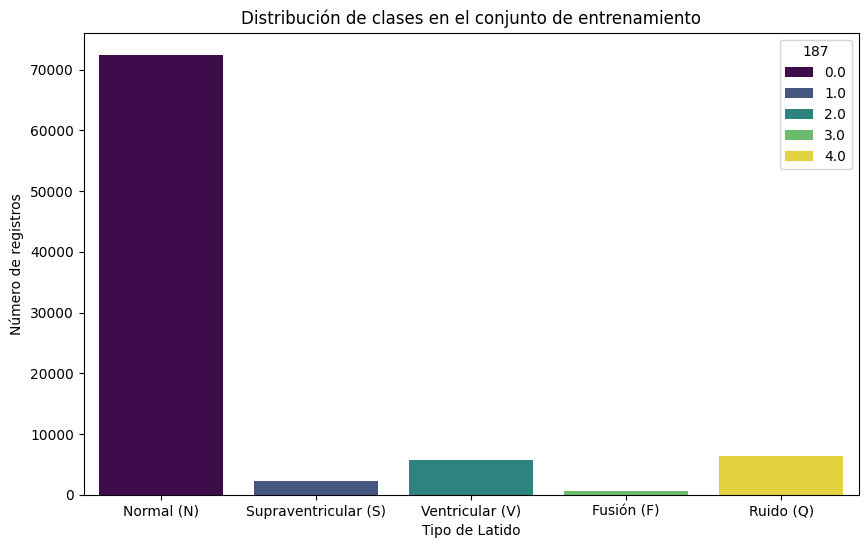
\includegraphics[width=0.8\columnwidth]{distr.png}
			\caption{Distribución de los tipos de latidos}
			\label{fig:distribucion}
		\end{figure}

		Primeramente, se comenzó analizando la distribución de amplitudes y valores atípicos por clase a través de boxplots, como se observa en Figura \ref{fig:ampl}, donde se observa
		un solapamiento en las distribuciones de todas las clases. Esto indica que la amplitud absoluta por sí sola no es suficiente para predecir arritmias, sino que es necesario
		observar en detalle la forma de la onda a lo largo del tiempo para identificar patrones sobre la misma que distingan las clases correctamente.

		\begin{figure}[H]
			\centering
			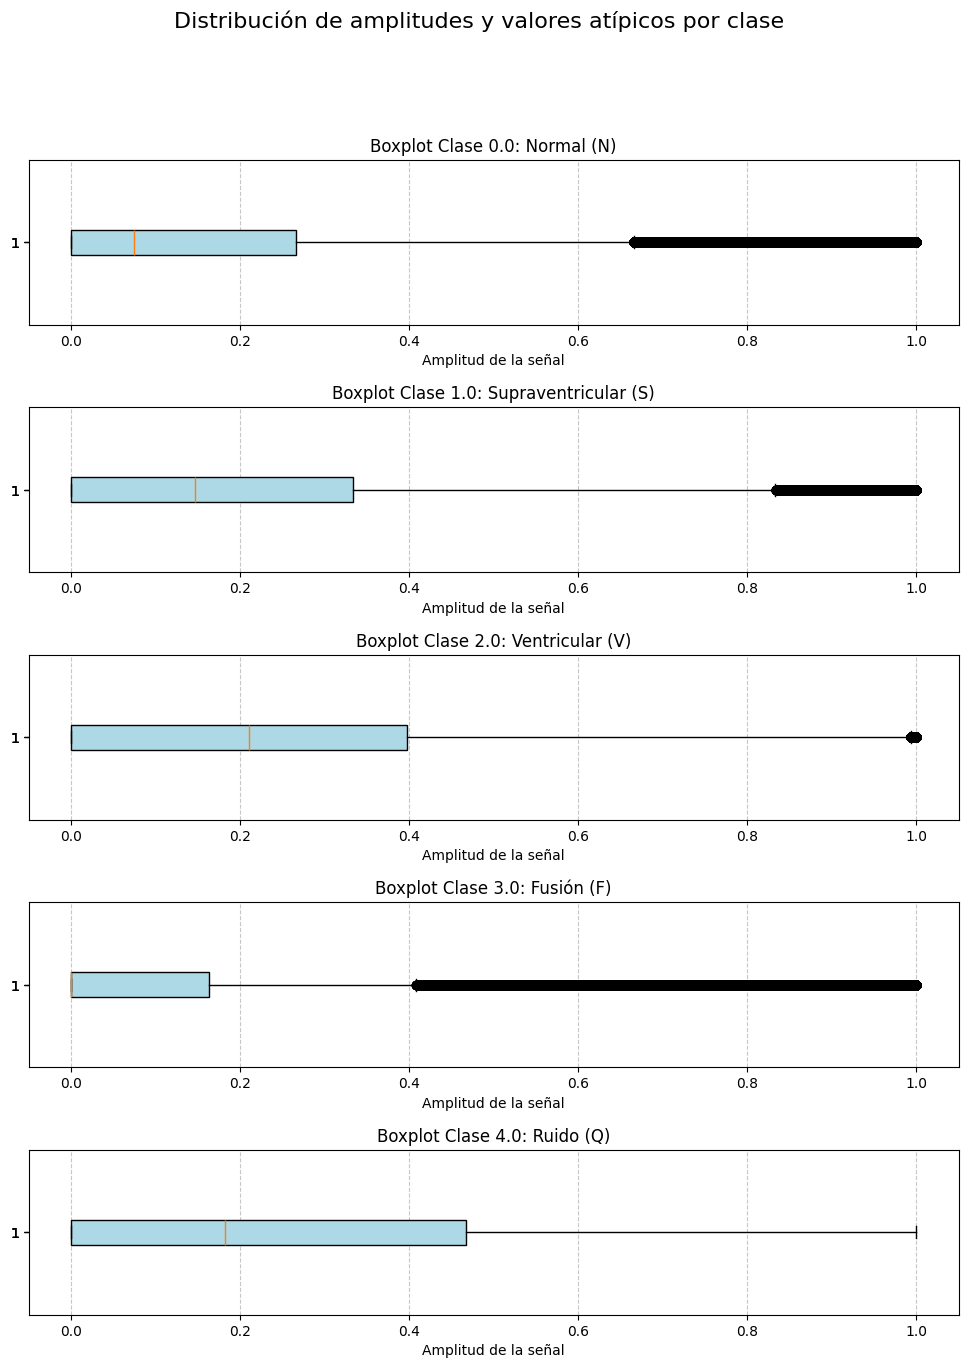
\includegraphics[width=0.8\columnwidth]{distr_ampl.png}
			\caption{Distribución de la amplitud}
			\label{fig:ampl}
		\end{figure}

		\vspace{0.2cm}

		A continuación, se graficaron las trayectorias temporales de amplitud promedio con bandas de dispersión (media ± 1 desviación estándar) para cada clase.
		El resultado, fue el obtenido en Figura \ref{fig:graf}, donde a pesar de que a simple vista no se aprecian de forma notable diferencias, se observan pequeños picos
		que denotan diferencias sutiles en el tipo que identifican latidos anómalos, como es el caso de los latidos de tipo fusión, que muestran un pico secundario muy
		claro alrededor de la muestra 60, la clase ventricular, cuya caída inicial es menos brusca y el sombreado es más ancho, lo cual indica una variabilidad más alta en sus
		latidos, o la clase supraventricular, que tiene un segundo pico cerca de la muestra 90 que los latidos normales no presentan.

		\begin{figure}[H]
			\centering
			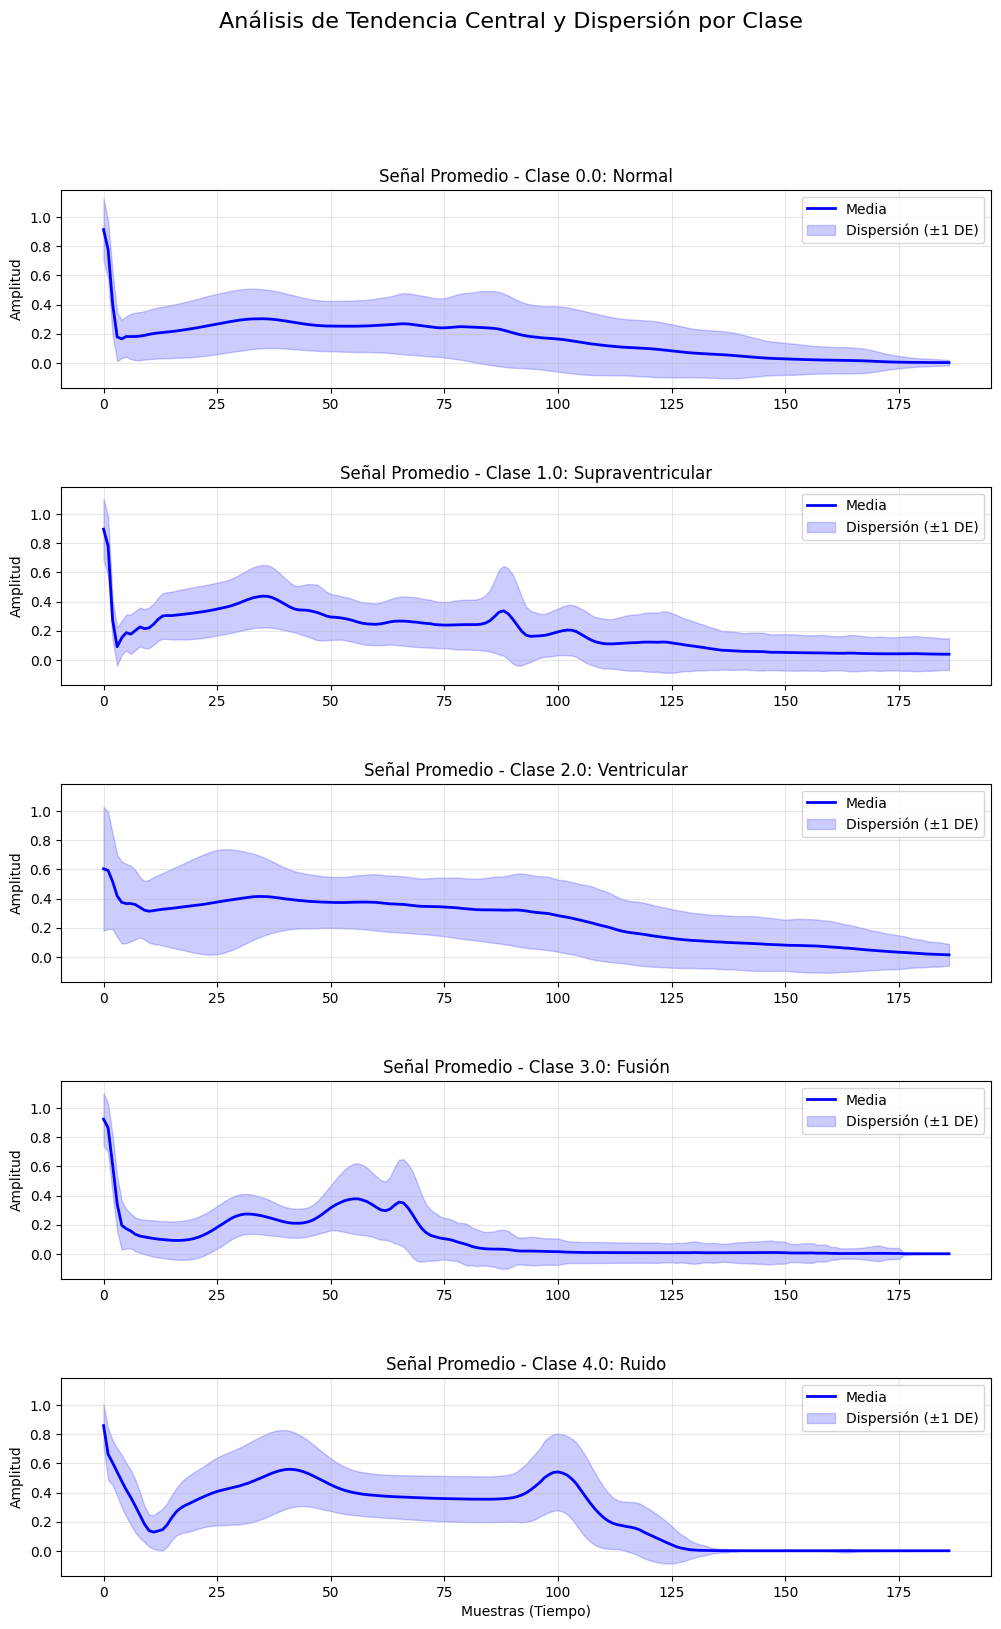
\includegraphics[width=0.8\columnwidth]{grafica_latidos1.png}
			\caption{Variabilidad dentro de cada tipo de latido}
			\label{fig:graf}
		\end{figure}
 
		\vspace{0.2cm}

	\section{Reducción de Dimensionalidad (PCA)}
	\label{sec:pca}

	El dataset de características ECG comprende 187 dimensiones, por lo que el Análisis de Componentes Principales (PCA) es una técnica fundamental a fin de reducir la dimensionalidad
	con el objetivo de identificar patrones, relaciones o estructuras en el espacio reducido de características.

	\vspace{0.2cm} 

	Un pre-requisito crítico es la estandarización de todas las características, y a pesar de que el dataset original contiene valores aproximadamente normalizados en escala [0, 1], el algoritmo PCA es extremadamente sensible a diferencias en rangos y varianzas entre características. Sin estandarización, características con mayores rangos dominarían los primeros componentes principales, sesgando así el análisis.

	\vspace{0.2cm} 

	Una vez estandarizadas las características, se aplicó PCA, reduciendo así el espacio a dos componentes principales para permitir la visualización bidimensional de la separabilidad entre clases. Los resultados mostraron:

	\vspace{0.2cm}

	\begin{itemize}
		\item \textbf{Componente Principal 1 (PC1):} Explica un 36.63\% de la varianza total.
		\item \textbf{Componente Principal 2 (PC2):} Explica un 15.63\% de la varianza total.
		\item \textbf{Varianza acumulada (PC1 + PC2):} Aproximadamente 52.26\% de la varianza total.
	\end{itemize}

	\vspace{0.2cm}

	Las cifras mostradas anteriormente, indican que casi el 50\% de la información discriminativa entre los tipos de latidos se encuentra en dimensiones superiores del espacio de características,
	por lo que se está perdiendo información por el camino. Esto, explica el solapamiento entre las clases observado en la representación bidimensional de ambos componentes que se mostrará a continuación. 

	\vspace{0.2cm}

	La visualización en el espacio de PC1-PC2 mostrada en Figura \ref{fig:pca} muestra un solapamiento significativo entre todas las cinco clases, lo cual indica la necesidad de usar
	el espacio completo de características para lograr una sensibilidad diagnóstica clínicamente aceptable, que dado la grave implicación que puede suponer un diagnóstico erróneo, es crítica
	una precisión más que aceptable. Además, la figura demuestra que las características discriminantes entre arritmias no se encuentran en un número reducido de dimensiones, sino a lo largo
	de detalles en el espectro de la señal a los que los métodos lineales simples no son capaces de llegar, requiriendo así métodos de separación no-lineal.


	\begin{figure}[H]
		\centering
		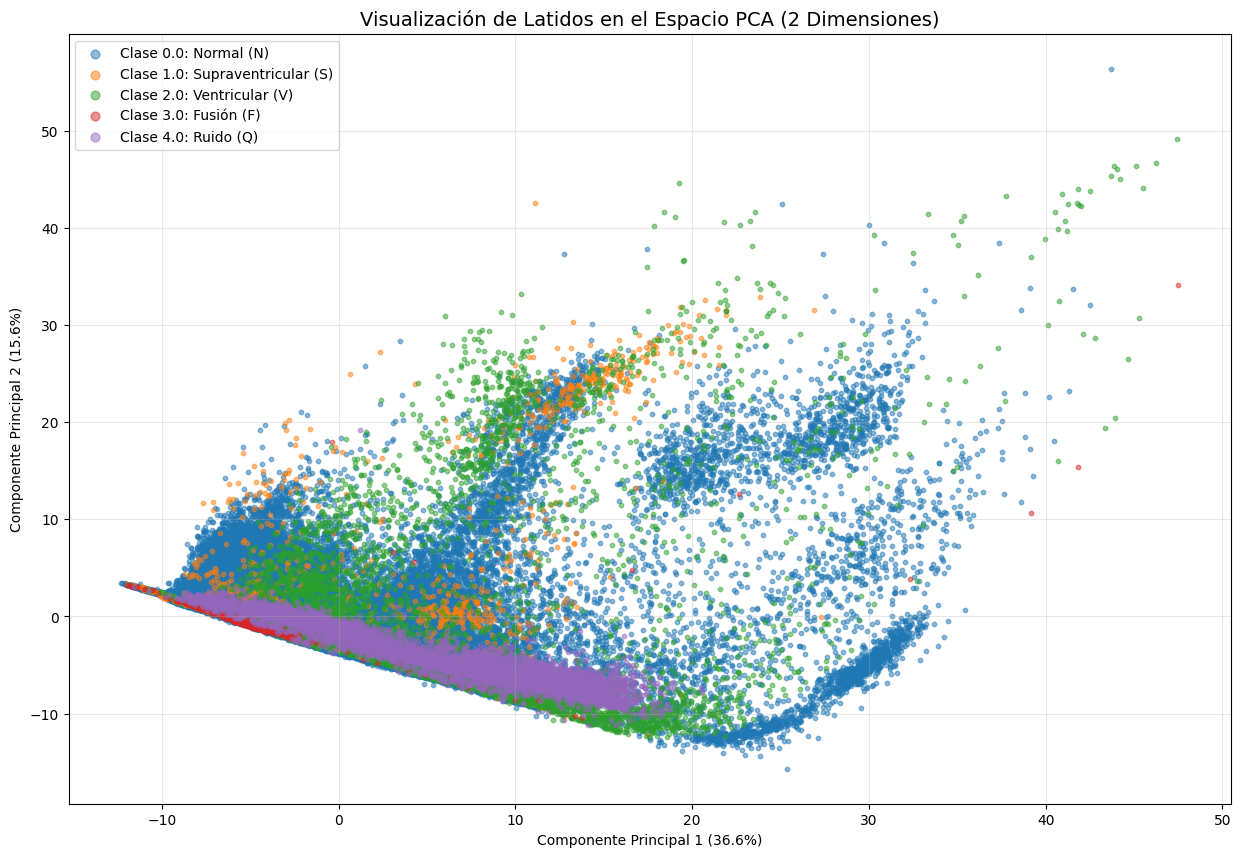
\includegraphics[width=0.8\columnwidth]{pca.png}
		\caption{Visualización de los tipos de latidos en el espacio PCA (2 dimensiones)}
		\label{fig:pca}
	\end{figure}

	\vspace{0.2cm}

	\section{Modelos de clasificación}
	\label{sec:modelos}

	En este apartado se entrenaron dos modelos de clasificación supervisada con base estadística, que fueron aplicados a los datos de latidos: (1) un árbol de decisión, que captura particiones no-lineales del espacio de características mediante búsqueda greedy, y (2) un clasificador bayesiano gaussiano, que modela la densidad probabilística de cada clase asumiendo distribuciones normales multivariadas.
	
	\vspace{0.2cm}

	Como se observó anteriormente, existe un grave problema que ha de tenerse en cuenta, y es el desbalanceo entre las clases, ya que con una distribución 82.77\% normales y 0.73\% fusión, un algoritmo que ignorara la estructura
	de los datos obtendría una alta precisión. Por lo que para la elección y confección de los modelos se ha tenido esto en cuenta al evaluar el desempeño de los mismos mediante métricas específicas
	y no mediante precisión global.

	\subsection{Árbol de Decisión}

	Un árbol de decisión particiona el espacio de características mediante una serie de umbrales binarios, con el objetivo de maximizar la homogeneidad diagnóstica dentro de cada región terminal. 
	Para compensar el desbalanceo de los datos, se implementó el parámetro \texttt{class\_weight="balanced"}.

	\vspace{0.2cm}
	
	Se entrenó un árbol de decisión con profundidad máxima de 10 nodos para evitar overfitting.

	\subsection{Clasificador Bayesiano Gaussiano}

	El clasificador bayesiano gaussiano (Naive Bayes) modela cada clase como una distribución normal multivariada en el espacio de características. Para una clase $c$, asume que cada característica es independiente dada la etiqueta de clase:

	\[
	P(c | \mathbf{x}) \propto P(\mathbf{x} | c) \cdot P(c) = \prod_{i=1}^{d} P(x_i | c) \cdot P(c)
	\]

	donde $P(c)$ es la probabilidad a priori (proporción de la clase en el conjunto de entrenamiento), y $P(x_i | c)$ es una distribución normal con media $\mu_{c,i}$ y varianza $\sigma^2_{c,i}$.

	\subsection{Evaluación y validación}

	Ambos modelos fueron entrenados sobre el conjunto de entrenamiento completo (87,554 muestras) y evaluados sobre el conjunto de validación (21,892 muestras). Las métricas de desempeño comprenden:

	\begin{enumerate}
		\item \textbf{Matriz de confusión:} Matriz de 2×2 donde entrada $(i,j)$ representa el número de muestras de la clase real $i$ predichas como clase $j$.
		
		\item \textbf{Precisión global:} $\text{Accuracy} = \frac{\text{ correctas}}{\text{ total}}$. Métrica de resumen, pero sesgada en presencia de desbalanceo.
		
		\item \textbf{Sensibilidad por clase:} $\text{Recall}_c = \frac{\text{TP}_c}{\text{TP}_c + \text{FN}_c}$. Proporción de muestras verdaderas de la clase $c$ correctamente identificadas, la cual es crítica para detectar arritmias raras.
		
		\item \textbf{Especificidad por clase:} $\text{Specificity}_c = \frac{\text{TN}_c}{\text{TN}_c + \text{FP}_c}$. Proporción de muestras no-clase-$c$ correctamente rechazadas.
		
		\item \textbf{Puntuación F1:} $\text{F1}_c = 2 \cdot \frac{\text{Precision}_c \cdot \text{Recall}_c}{\text{Precision}_c + \text{Recall}_c}$. Media armónica de precisión y recall, relevante cuando el desbalanceo es importante.
	\end{enumerate}

	\vspace{0.2cm}

Como a pesar de que existen 5 etiquetas que definen los distintos tipos de latidos y realmente se está evaluando la anomalía de los mismos, se transformó el problema en uno de clasificación binaria, donde la clase 0 (latido normal) se mantendrá y las clases 1 a 4 (latidos anómalos) se agruparán en una única clase 1 (latido anómalo). Estas etiquetas binarias se emplearán para entrenar y evaluar los modelos.
	%================================================

	\section{Resultados}
	\label{sec:resultados}

	\subsection{Desempeño del Árbol de Decisión}

Como se observa en la tabla resumen Tabla \ref{tab:arbol_resultados}, el árbol de decisión demostró una alta eficacia clínica al alcanzar una sensibilidad (recall) del 88\% en la detección de latidos anómalos. 
Si bien la precisión del 82\% indica la existencia de falsos positivos (latidos normales clasificados erróneamente como anómalos), este comportamiento es preferible en un dispositivo de salud.
Dado que el objetivo del wearable es alertar ante la presencia de posibles arritmias, se prioriza minimizar los falsos negativos (enfermos no detectados), ofreciendo un balance aceptable.

	\vspace{0.2cm}

	\begin{table}[H]
		\centering
		{\small
		\caption{Métricas de desempeño del Árbol de Decisión por clase diagnóstica.}
		\label{tab:arbol_resultados}
		\setlength{\tabcolsep}{6pt}
		\begin{tabular}{|l|c|c|c|}
			\hline\hline
			\textbf{Clase} & \textbf{Precisión} & \textbf{Sensibilidad} & \textbf{F1-Score} \\\hline
			(N) & 0.97 & 0.96 & 0.97 \\\hline
			(A) & 0.82 & 0.88 & 0.85 \\\hline\hline
		\end{tabular}
		}
	\end{table}

	\vspace{0.2cm}

	A continuación, se presenta la matriz de confusión en la Figura \ref{fig:confusion_mat}, donde se observa cómo el modelo logra 
	separar eficazmente la clase mayoritaria (Normal), manteniendo un alto índice de acierto en la clase Anómala a pesar del 
	desbalanceo original de los datos. Los errores observados (falsos positivos) son una consecuencia esperada del solapamiento de 
	características visualizado previamente en el PCA, pero no comprometen la utilidad del sistema como herramienta de alerta temprana.

	\begin{figure}[H]
		\centering
		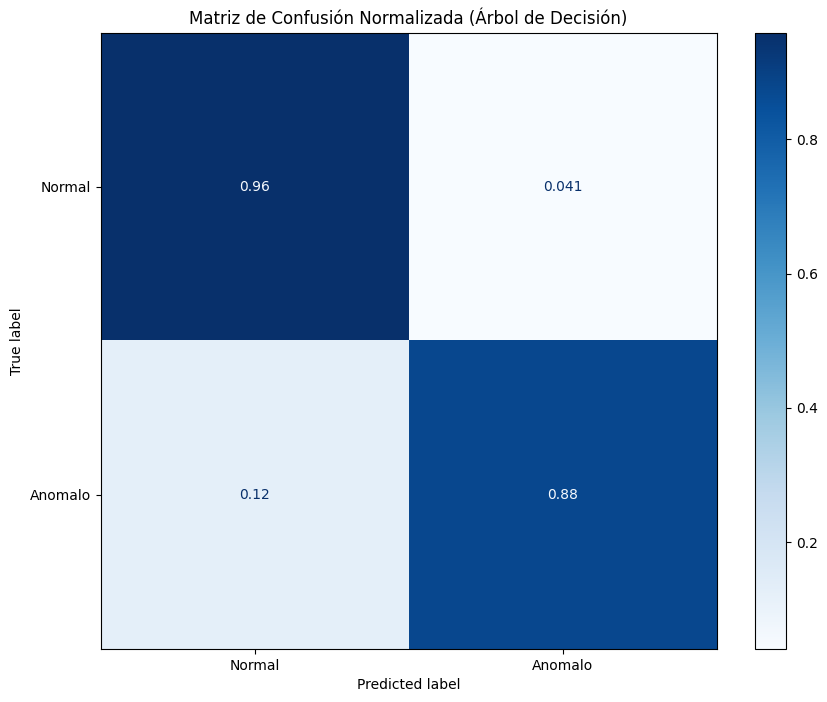
\includegraphics[width=0.8\columnwidth]{confusion_mat.png}
		\caption{Matriz de Confusión para el Árbol de Decisión}
		\label{fig:confusion_mat}
	\end{figure}

	\subsection{Desempeño del Clasificador Bayesiano Gaussiano}

Como se evidencia en la Tabla \ref{tab:gaussiano}, el clasificador Naive Bayes muestra un rendimiento muy inferior al Árbol de Decisión, resultando ineficaz para este caso clínico. 
Su principal fallo radica en la baja sensibilidad (Recall) del 49\% para la clase anómala. Esto significa que el modelo es incapaz de detectar más de la mitad de las arritmias reales (Falsos Negativos), lo cual viola la premisa fundamental de seguridad del wearable. Además, su precisión del 45\% indica que, cuando alerta, se equivoca más de la mitad de las veces.

	\vspace{0.2cm}

	El motivo por el cual Naive Bayes no funciona es precisamente por la asunción de independencia, ya que este modelo asume que cada uno de los 187 puntos del ECG es independiente del resto,
	ignorando así la estructura temporal de la señal, que es vital para el diagnóstico. Además, la suposición de distribuciones gaussianas no son válidas para todas las clases.

	
	\begin{table}[H]
		\centering
		{\small
		\caption{Métricas de desempeño del Clasificador Bayesiano Gaussiano.}
		\label{tab:gaussiano}
		\setlength{\tabcolsep}{6pt}
		\begin{tabular}{|l|c|c|c|}
			\hline\hline
			\textbf{Clase} & \textbf{Precisión} & \textbf{Sensibilidad} & \textbf{F1-Score} \\\hline
			(N) & 0.89 & 0.88 & 0.88 \\\hline
			(A) & 0.45 & 0.49 & 0.47 \\\hline\hline
		\end{tabular}
		}
	\end{table}

	\vspace{0.2cm} 

Complementando la información anterior, la matriz de confusión en la Figura \ref{fig:bayes} confirma la incapacidad del modelo para 
separar las dos clases. A diferencia del árbol, que lograba aislar bien a los pacientes sanos, el modelo Bayesiano genera un número 
inaceptable tanto de Falsos Negativos (enfermos mandados a casa) como de Falsos Positivos.
	
	\begin{figure}[H]
		\centering
		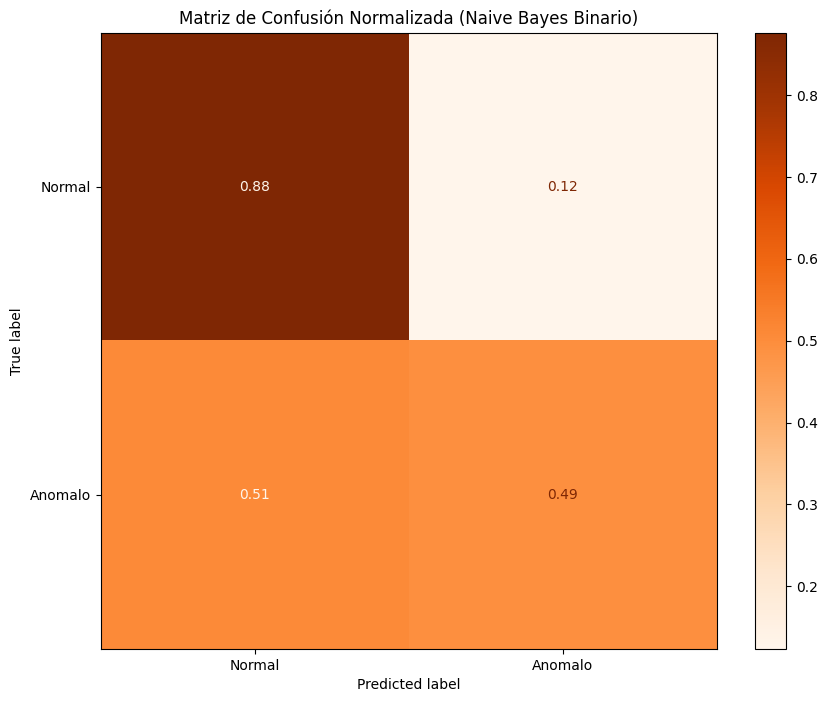
\includegraphics[width=0.8\columnwidth]{conf_mat_bayes.png}
		\caption{Matriz de Confusión Naive-Bayes}
		\label{fig:bayes}
	\end{figure}

	\section{Probabilidades Condicionales y Teorema de Bayes}

	En este apartado se evalúa la capacidad de un patrón para predecir la presencia de una arritmia ventricular (Clase 2), utilizando el Teorema de Bayes para calcular la probabilidad a posteriori,
	análisis fundamental para determinar la viabilidad del sistema de alertas para el \textit{wearable}.

	\subsection{Definición del Patrón de Interés ($X$)}
	Para el desarrollo de este análisis, se ha definido el \textbf{Patrón $X$} como una amplitud de señal superior a $0.3$ en la muestra de tiempo $3$ ($t_{3} > 0.3$), basándose 
	en el análisis descriptivo previo, donde se observó que los latidos de la \textbf{Clase 2 (Ventricular)} presentan una amplitudes sostenida en esta 
	fase de la onda en comparación con el latido cardiaco normal.

	\subsection{Cálculo de Probabilidades y Aplicación del Teorema}
	A continuación, a partir de los datos del conjunto de entrenamiento, se aplicó la fórmula de Bayes para determinar la probabilidad de que un latido sea una arritmia dado que presenta el patrón mencionado:

	\begin{equation}
	P(\text{Clase 2} | X) = \frac{P(X | \text{Clase 2}) \cdot P(\text{Clase 2})}{P(X)}
	\end{equation}

	A partir del procesamiento de los datos, se obtuvieron los siguientes valores probabilísticos:

	\begin{itemize}
		\item \textbf{Probabilidad a Priori $P(\text{Clase 2})$:} \textbf{0.0661} (Refleja la baja prevalencia de esta arritmia en el dataset).
		\item \textbf{Verosimilitud $P(X | \text{Clase 2})$:} \textbf{0.5195} (Frecuencia con la que el patrón $X$ aparece en latidos ventriculares).
		\item \textbf{Evidencia $P(X)$:} \textbf{0.2969} (Probabilidad marginal de observar el patrón en cualquier tipo de latido).
	\end{itemize}

	Sustituyendo estos valores, se obtuvo una probabilidad a posteriori de:
	\begin{center}
		\textbf{$P(\text{Clase 2} | X) = $ 0.1157}
	\end{center}

	\subsection{Interpretación de Resultados y Riesgo Clínico}
	
	Al aplicar el Teorema de Bayes, los resultados indican que a pesar de que la aplicación del mismo es útil, un sistema de alerta que se basa en un
	único umbral está destinado a equivocarse constantemente, produciendo interrupciones al usuario 9 de cada 10 veces. Esto hace que sea estrictamente
	necesaria la aplicación de modelos de Machine Learning como el árbol de decisión implementado anteriormente, que combina múltiples umbrales
	para mantener una alta sensibilidad, reduciendo así los falsos positivos.

	\section{Conclusiones}
	\label{sec:conclusiones}

	Una vez estudiada la viabilidad del wearable, se obtuvieron las siguientes conclusiones:

	\begin{enumerate}
		\item \textbf{Desafío del desbalanceo:} La distribución de los diagnósticos muestra un predominio de latidos normales (82.77\%) sobre patologías (máximo 8.09\% para supraventriculares), por lo que la complejidad se encuentra en no omitir las patologías minoritarias.
		
		\item \textbf{Complejidad alta:} El análisis PCA reveló que solo el 52.26\% de la varianza se explica con los componentes principales, lo que obliga a utilizar todas las características de la señal para una clasificación efectiva.
				
		\item \textbf{Modelos complementarios:} El árbol de decisión ofrece interpretabilidad de características clave, mientras que el clasificador bayesiano proporciona cuantificación de confianza diagnóstica.
	\end{enumerate}

	A pesar del solapamiento entre las clases, los modelos entrenados superaron las expectativas iniciales, demostrando la viabilidad de este tipo de sistemas de medicina preventiva.
	
	\end{document}